\section{Methods}
\label{S:4}

We investigated different blockchain implementations and compared their features to gain insight in to what would be the most suitable solution. We eventually decided upon Ethereum as it offers a Turing-complete language for smart contracts along with a great community of developers and extensive documentation. Of course, this choice has some side effectes, in this section we describe our steps in making this decision and the implementation of the system.  

After having chosen the blockchain implementation and explained the new design, we describe the setup for the performance tests.

\subsection{Choosing the blockchain}

The choice of the most appropriate blockchain technology should take into account:
\begin{itemize}
  \item \textbf{Acknowledged security}: the blockchain should not contain any technical flaw and be recognized by the community as \textit{trustable}\footnote{The authors realise that this concept is abstract and often biased, in order to evaluate the \textit{trustability}, github stars (when available) and blockchain market capitalization value (when available) have been analysed} . This is important since many projects are based on a good and promising concept but often times fail on the practical implementation.
  \item \textbf{Production stage}: many blockchains on the market are still young and immature. This problem is probably due to the fact that investors want to quickly enter the market, creating overhead and confusion to the third party services that embrace a yet-not-ready product.
  \item \textbf{Contract execution}: the execution of the contracts allows developers to define rules (e.g. which authorities are able to change a GlobalId and the modalities of such operations).
  \item \textbf{Decentralized Control}: since it is a blockchain prerogative, the technology should not be owned by a restricted group of actors and everyone must be able to join at will. This will avoid any conflict of interest or predominance among the parties.
\end{itemize}

In table \ref{Table:1} we analyse the most well-known blockchains.

\begin{table}[h!]
\centering
\caption{Comparison of different blockchains}
\label{Table:1}
\begin{tabular}{ |p{7cm}|p{2cm}|p{2cm}|p{2cm}|p{2cm}|  }
\hline
\multicolumn{5}{|c|}{Chosing the blockchain} \\
\hline
Blockchain candidate & Security & Production Stage & Contract Execution & Public \\
\hline
Bitcoin and AltCoins \cite{nakamoto_bitcoin_2008} & Yes & Yes & No & Yes \\
\hline
Ethereum \cite{wood_ethereum_2014} & Yes & Yes & Yes & Yes \\
\hline
BigchainDB \cite{bigchaindb_whitepaper} & No \cite{_bigchaindb_bullshit} \ & No & Yes & Yes \\
\hline
Lisk (not whitepaper available a.t.m., please refer to https://lisk.io/) & Yes & No \cite{lisk_problems} & Yes & Yes \\
\hline
IOTA \cite{iota_whitepaper}& No \cite{iota_problems} & No & Yes & Yes \\
\hline
Hyperledger Fabric \cite{martindale_fabric:_2017}& Yes & Yes & Yes & No \\
\hline
R3 Corda \cite{corda_whitepaper}& Yes & Yes & Yes & No \\
\hline
\end{tabular}
\end{table}

\FloatBarrier
The features provided by Ethereum technology seem to be the ones that most fit our necessities enabling us to replace the previous DHT system. The main reasons we choose this specific blockchain technology are:

% \begin{notation}
%   TODO: \\
%   Explain why ethereum and make comaprison with bitcoin (simply: bitcoin is expensive and non optimazed for key value. Other blockchain are not safe => bigchaindb or not yet fully developed => Lisk).

%   Other blockchain are not worth to be mention for lack of documentation.

%   How to explain this without sources if not the persona experience??
% \end{notation}

\begin{itemize}
  \item \textbf{Consistent storage by definition}: Ethereum blockchain creates different replicas of the same database in each node of the network. With such a solution, nodes can enter or exit the network without compromising any SR.
  \item \textbf{Recovery from failure}: In case of failure, it is possible to recover the state of the database and re-execute the missing transactions (pulling the transactions from the peers).
  \item \textbf{Consistency}: Ethereum is a distributed ledger hence, it is not possible to forge part of the database (at least 50\% + 1 of the nodes must be corrupted \cite{dennis_rep_2015}). This prevents any node from sending misleading SRs.
  \item \textbf{Scalability}: One of the main features of the blockchain is its endless scalability: thus we can set up large number of nodes (multiple GSLS servers for each OSN and for those users who are willing to set up one node) without facing any delay.
  Even better, increasing the size of the network and therefore the difficulty of a rewrite attack due to the requirement for compromising the 50\% + number of nodes.
  \item \textbf{Fast look up}: Hosting one node allows an entity to locally access the SRs stored into the GSLS storage. In contrast, in the previous implementation (with DHT) it was possible that one specific SR was only available in nodes far away from the requesting resource, creating a delay in the delivery of the information. 
\end{itemize}

Given these premises, Ethereum blockchain seems to be the most appropriate tool for the job: providing a consistent, distributed and scalable environment; accessible by all the players at the same time.


\subsection{Ethereum ecosystem}
\label{ethereumEcosystem:1}

Ethereum is an \textit{account model} blockchain \cite{wood_ethereum_2014}, therefore it is different from the mainstream \textit{Unspent transactions model (UTXO model)}  (such as the Bitcoin blockchain). This alternative implementation allows the blockchain to save memory space since the balance is kept in the account state (a key-value storage mapping addresses to an account state object \cite{ethereum_yellowpaper}) rather than keeping track of all the transaction changes (utxo) generated by one account in the blockchain itself.

A blockchain can be seen as a system that shifts from a state $t$ ($\sigma_t$) to a state $t+1$ ($\sigma_{t+1}$) due to the transactions $[t_0,t_1,...,t_n]$ (where $n$ is the number of the transaction $n-1$) stored into the block $B$ (Table\ref{table:2}).


\begin{table}[h!]
\centering
\caption{Basic structure of an Ethereum block}
\begin{tabular}{ |p{3cm}|  }
\hline
\multicolumn{1}{|c|}{Block structure} \\
\hline
\hline
Header \\
\hline
Transactions $[t_0,t_1,...,t_n]$ \\
\hline
Headers of onners blocks\\
\hline
\end{tabular}
\label{table:2}
\end{table}

Once the block is mined, is broadcasted and each node at state $t$  executes, through the EVM, each transaction inside the block in order.
This algorithm allows the nodes to eventually converge to the same state $t+1$ at some point in time.

Building the transaction is out of the scope of the EVM: this operations is delegated to the human being who owns the account or any sort of software/wallet she decides to employ.

There are two types of transactions: \textit{account creation} and \textit{message call to existing account}. Although these two types are conceptually distant, they share the same structure as they both include the following:

\begin{itemize}
  \item \textbf{nonce}: number of transactions sent from the sender account
  \item \textbf{gasPrice}: number of wei (smallest monetary unit) to pay per each unit of gas (virtual fuel needed to execute the transaction).
  \item \textbf{gasLimit}: maximum amount of gas that shall be used to execute the current transaction
  \item \textbf{to}: address of the account of the receiver
  \item \textbf{value}: number of wei assigned to the transaction
  \item \textbf{v, r, s}: Value of the transaction signature, this parameters are used to recover the sender's signature \cite{gura2004comparing}
  \item \textbf{init}: field with unlimited size; here the initialisation commands are specified directly in EVM code. This field is analysed only if the \textit{to} field is left empty
  \item \textbf{data}: field with unlimited size, specify the input data of the message call
\end{itemize}

Is trivial to notice that among all these fields the \textit{v}, \textit{r}, and \textit{s} are the most private ones; on this observation we create a workflow which allows the sender create and upload transactions even when an internet connection is unavailable. 

\subsubsection{Serializability of the Ethereum transaction}
Each user has a public key and a private key. It is possible to infer the public key starting from the private key; so that, given a random sequence of bytes (seed) is possible to create the key pair \cite{ethereum_yellowpaper}.

The account address is just the last 160 bits of the public key hashed via SHA3-256 \cite{sha3_256_keccak}.

Once the values of the transaction are set: \textit{nonce}, \textit{gasPrice}, \textit{gasLimit}, \textit{to} (can be left empty if is a new contract), \textit{value}, and \textit{data} is possible to serialise the transaction via recursive length prefix (RLP) \cite{wood_ethereum_2014} and hash it. Then the hash is signed with the private key, generating \textit{v}, \textit{r}, \textit{s}.

\subsection{Verify correctness of the transaction}
Once the transaction is ready, it can be uploaded to the network and mined. When the EVM executes it, it will perform the following operations in order:
\begin{enumerate}
  \item Verify that the RLP serialisation is not corrupted (no bytes at the end of the bytestream).
  \item Verify the transaction signature, recovering the public key from \textit{v}, \textit{r}, \textit{s} and finding the transaction hash; then comparing it with the RLP hash of the data received.
  \item Verify the validity of the \textit{nonce}, this operation can only be done after the public key has been recovered.
  \item Verify that the units of gas are sufficient to complete the transaction.
  \item Verify that the sender's balance is sufficient to execute the transaction ($gasPrice * gasLimit$).
\end{enumerate}

As showed, the transaction is serialised and encrypted when is uploaded to the blockchain.
At this stage is not possible to decrypt it or change any fields. It is therefore possible to stream the bytes of the transaction from one device to another in a safe manner.
\\

\begin{figure}[h]
	\centering
  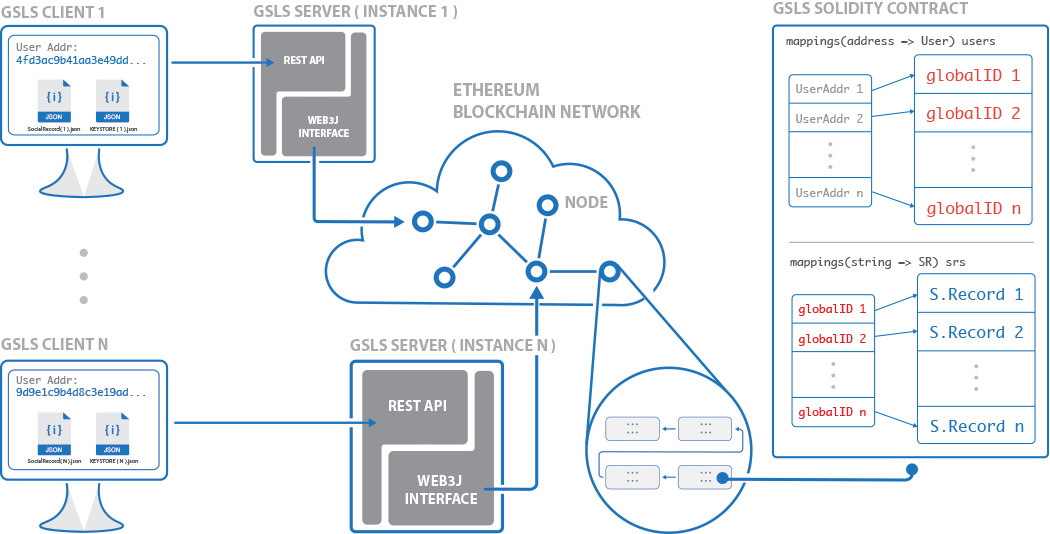
\includegraphics[width=1\textwidth]{gsls-architecture}
	\caption{Basic architecture: n clients communicate with m GSLS server instances. The GSLS instances can interface with the blockchain because each and every of them is holding an Ethereum node. All the operations are referenced to the contract address storing the list of SRs.}
	\label{fig4}
\end{figure}

\subsection{Performance Tests}

In order to make the tests possible, we created and deployed a smart contract on the Ethereum testnet, a blockchain with a simplified proof of work used by developers to test applications. Although the consensus is simplified, the mining time is comparable to the main public chain. 

The application was deployed in a single machine with 1 CPU and 4GB of RAM. Since the application relied on the distribution of blockchain, it was possible to use only a single machine, while the previous implementation needed to spawn at least three nodes to create the DHT \cite{gondor_distributed_2016}. The tested application also relied upon an on-line service to connect to an Ethereum blockchain node, although, in an ideal case, the GSLS server node should run a blockchain node. 

After having deployed the service, the tests were run in a similar fashion to the fist implementation of the GSLS. The service was tested on writing and reading times of the SR. To test the writing operation, 500 HTTP PUT and POST requests were sent to the service. The request body held the signed transaction with different \textit{gasPrices} and \textit{globalIDs}. To evaluate the performance of the reading operation, we sent 10000 HTTP GET requests to the service. All the request durations were logged and stored in a log file.


